\documentclass[aspectratio=169]{beamer}


% Beamer settings
\usecolortheme{rose}
\beamertemplatenavigationsymbolsempty
\setbeamertemplate{footline}[frame number]

\titlegraphic{%

\includegraphics[height=1cm]{logo-full-colour.png}}

\addtobeamertemplate{frametitle}{}{%
\begin{tikzpicture}[remember picture,overlay]
\node[anchor=north east,yshift=2pt] at (current page.north east) {
\includegraphics[height=1cm]{logo-full-colour.png}};
\end{tikzpicture}}

% Packages
\usepackage{amsmath}

\usepackage{tikz}
\usetikzlibrary{positioning}
\usetikzlibrary{fit}

\usepackage{pgfplots}
\usepgfplotslibrary{fillbetween}

\usepackage{minted}
\usepackage[T1]{fontenc} % Required by minted to ensure dollar signs are produced instead of pound (sterling) signs

\usepackage{multicol}

\usepackage{booktabs}

\usepackage{adjustbox}

% Author
\author{Simon McIntosh-Smith \& Tom Deakin\\University of Bristol}

\date{}



\title{OpenMP for Computational Scientists}
\subtitle{Preliminaries}

\begin{document}

\frame{\titlepage}

%-------------------------------------------------------------------------------
% \begin{frame}
% \frametitle{Audience}

% \begin{itemize}
% \item Teaches OpenMP 4.5 and 5.0 in a seminar style.
% \item 6 lecture topics, with exercises and solutions.
% \item Designed for Computational Scientists familiar with Fortran and MPI programming.

% \end{itemize}

% Download code (and slides) from:
% \url{https://github.com/UoB-HPC/openmp-for-cs}

% \end{frame}
%-------------------------------------------------------------------------------

\begin{frame}
\frametitle{Introduction}

\begin{itemize}
  \item Today: Learn OpenMP 4.5 (and maybe some 5.0).
  \item We will cover a lot of material!
  \item This is a hands-on tutorial!
  \item Mixture of lectures and exercises.
  % \item Exercises designed to try programming OpenMP.
  \item Experiment and have fun with them!
  \item Solutions provided, but only look as last resort.
  \item Assume knowledge of basic Fortran; parallel programming with MPI useful.
\end{itemize}
\end{frame}

%-------------------------------------------------------------------------------

\begin{frame}
\frametitle{Materials}
\begin{block}{Materials}
Download code (and slides) from:
\url{https://github.com/UoB-HPC/openmp-for-cs}
\end{block}
\end{frame}
%-------------------------------------------------------------------------------

\begin{frame}
\frametitle{GW4 Isambard}
\begin{columns}
  \begin{column}{0.7\framewidth}
    \begin{itemize}
      \item UK Tier-2 Supercomputer.
      \item Collaboration between GW4 Alliance, UK Met Office, Cray, Arm and EPSRC.
      \item 21,000+ Armv8 cores.
      \item Collection of CPUs/GPUs from different vendors.
      \item \textbf{Today:} using the Intel Xeon 2x18-core Broadwell and NVIDIA P100 nodes.
    \end{itemize}
  \end{column}
  \begin{column}{0.3\framewidth}
    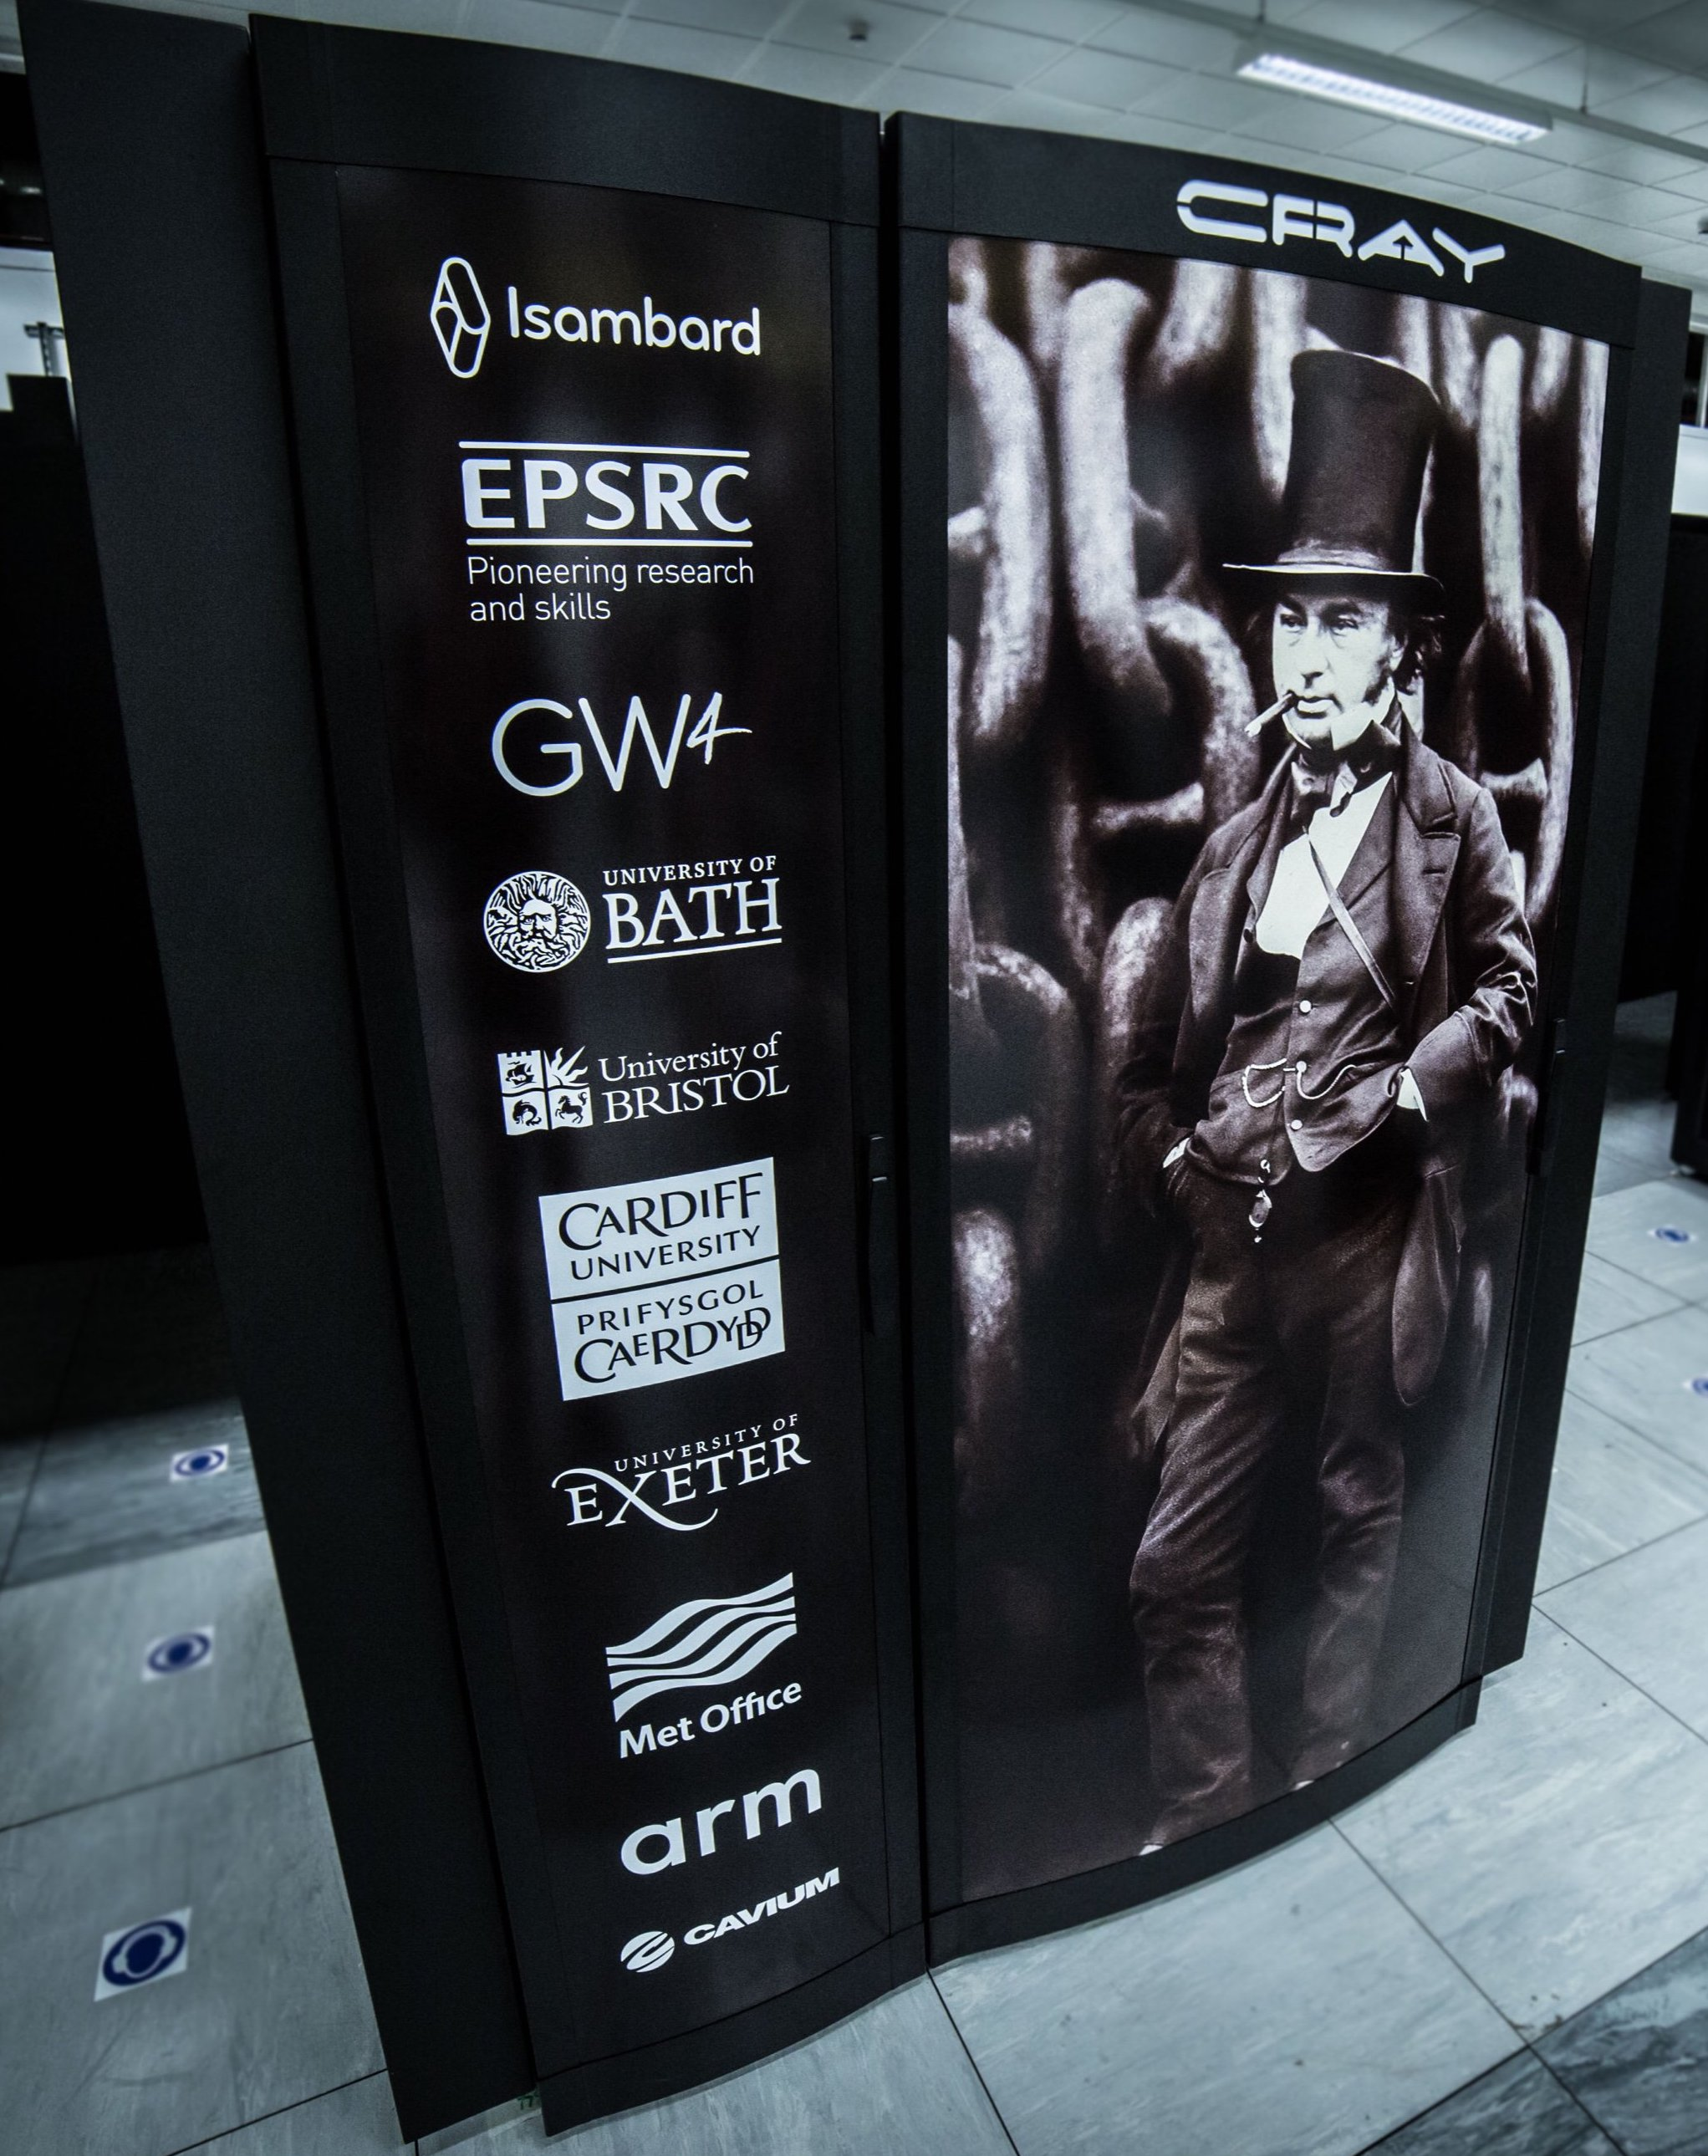
\includegraphics[width=\textwidth]{isambard.jpeg}
  \end{column}
\end{columns}

Thanks to Simon McIntosh-Smith and Bristol for supporting today's tutorial with time on Isambard.

\end{frame}

%-------------------------------------------------------------------------------


\begin{frame}
\frametitle{Agenda}

\textbf{Part One: CPUs}
\begin{description}
  \item[09:30--09:40] Introduction.
  \item[09:40--10:10] Parallel worksharing.
  \item[10:10--10:35] Exercise 1: Parallel stencil (two-ways).
  \item[10:35--11:00] Data sharing.
  \item[11:00--11:15] Coffee Break.
  \item[11:15--11:35] Exercise 2: Parallel convergence.
  \item[11:35--12:10] Vectorisation and NUMA.
  \item[12:10--12:30] Exercise 3: Optimising stencil.
\end{description}

\textbf{Lunch break (12:30--13:30)}
\end{frame}

\begin{frame}
\frametitle{Agenda}
\textbf{Lunch break (12:30--13:30)}
The Zoom session is open: feel free to continue on the morning exercises and ask questions in the Q and A.

\textbf{Part Two: GPUs}
\begin{description}
  \item[13:30--13:35] Welcome back.
  \item[13:35--14:10] Transferring execution and data movement.
  \item[14:10--14:35] Exercise 4: Stencil on a GPU.
  \item[14:35--15:00] Target Parallelism.
  \item[15:00--15:15] Coffee Break.
  \item[15:15--15:40] Optimising data movement.
  \item[15:40--16:25] Exercise 5: Optimising stencil on a GPU.
  \item[16:25--16:30] Wrap up.
\end{description}
\end{frame}

%-------------------------------------------------------------------------------

% \begin{frame}
% \frametitle{Exercises}
% \begin{itemize}
% \item This is a hands-on course!
% \item Exercises will be set for you to try programming OpenMP yourselves.
% \item Sample solutions also provided.
% \item All the exercises will be in Fortran.
% \end{itemize}

% \end{frame}

%-------------------------------------------------------------------------------
% \section{Outline}
% \begin{frame}
% \frametitle{Course Outline}
% Organised as 6 sessions teaching OpenMP plus top-tips for getting good performance.
% \begin{enumerate}
%   \item OpenMP overview
%   \item Data sharing and reductions
%   \item Vectorisation and code optimisations
%   \item NUMA and MPI interoperability
%   \item GPU programming with OpenMP
%   \item Tasks and Tools
% \end{enumerate}
% \end{frame}

%-------------------------------------------------------------------------------
\begin{frame}
\frametitle{Thanks}
Thanks go to the following authors, whose own OpenMP tutorials have inspired this one:
\begin{itemize}
  \item Tim Mattson (Intel)
  \item Alice Koniges (Berkeley Lab/NERSC)
  \item Simon McIntosh-Smith and the HPC team (UoBristol)
  \item Gethin Williams (UoBristol)
  \item and many others
\end{itemize}
\end{frame}
%-------------------------------------------------------------------------------

\end{document}
